\chapter{Application and validation}

After the theoretical basis of the virtual experiment platform is known and 
the program of the virtual experiment platform is built, the application should be 
verified with experiment data generated based on the real experiment.


\begin{figure}[htbp]
    \centering
    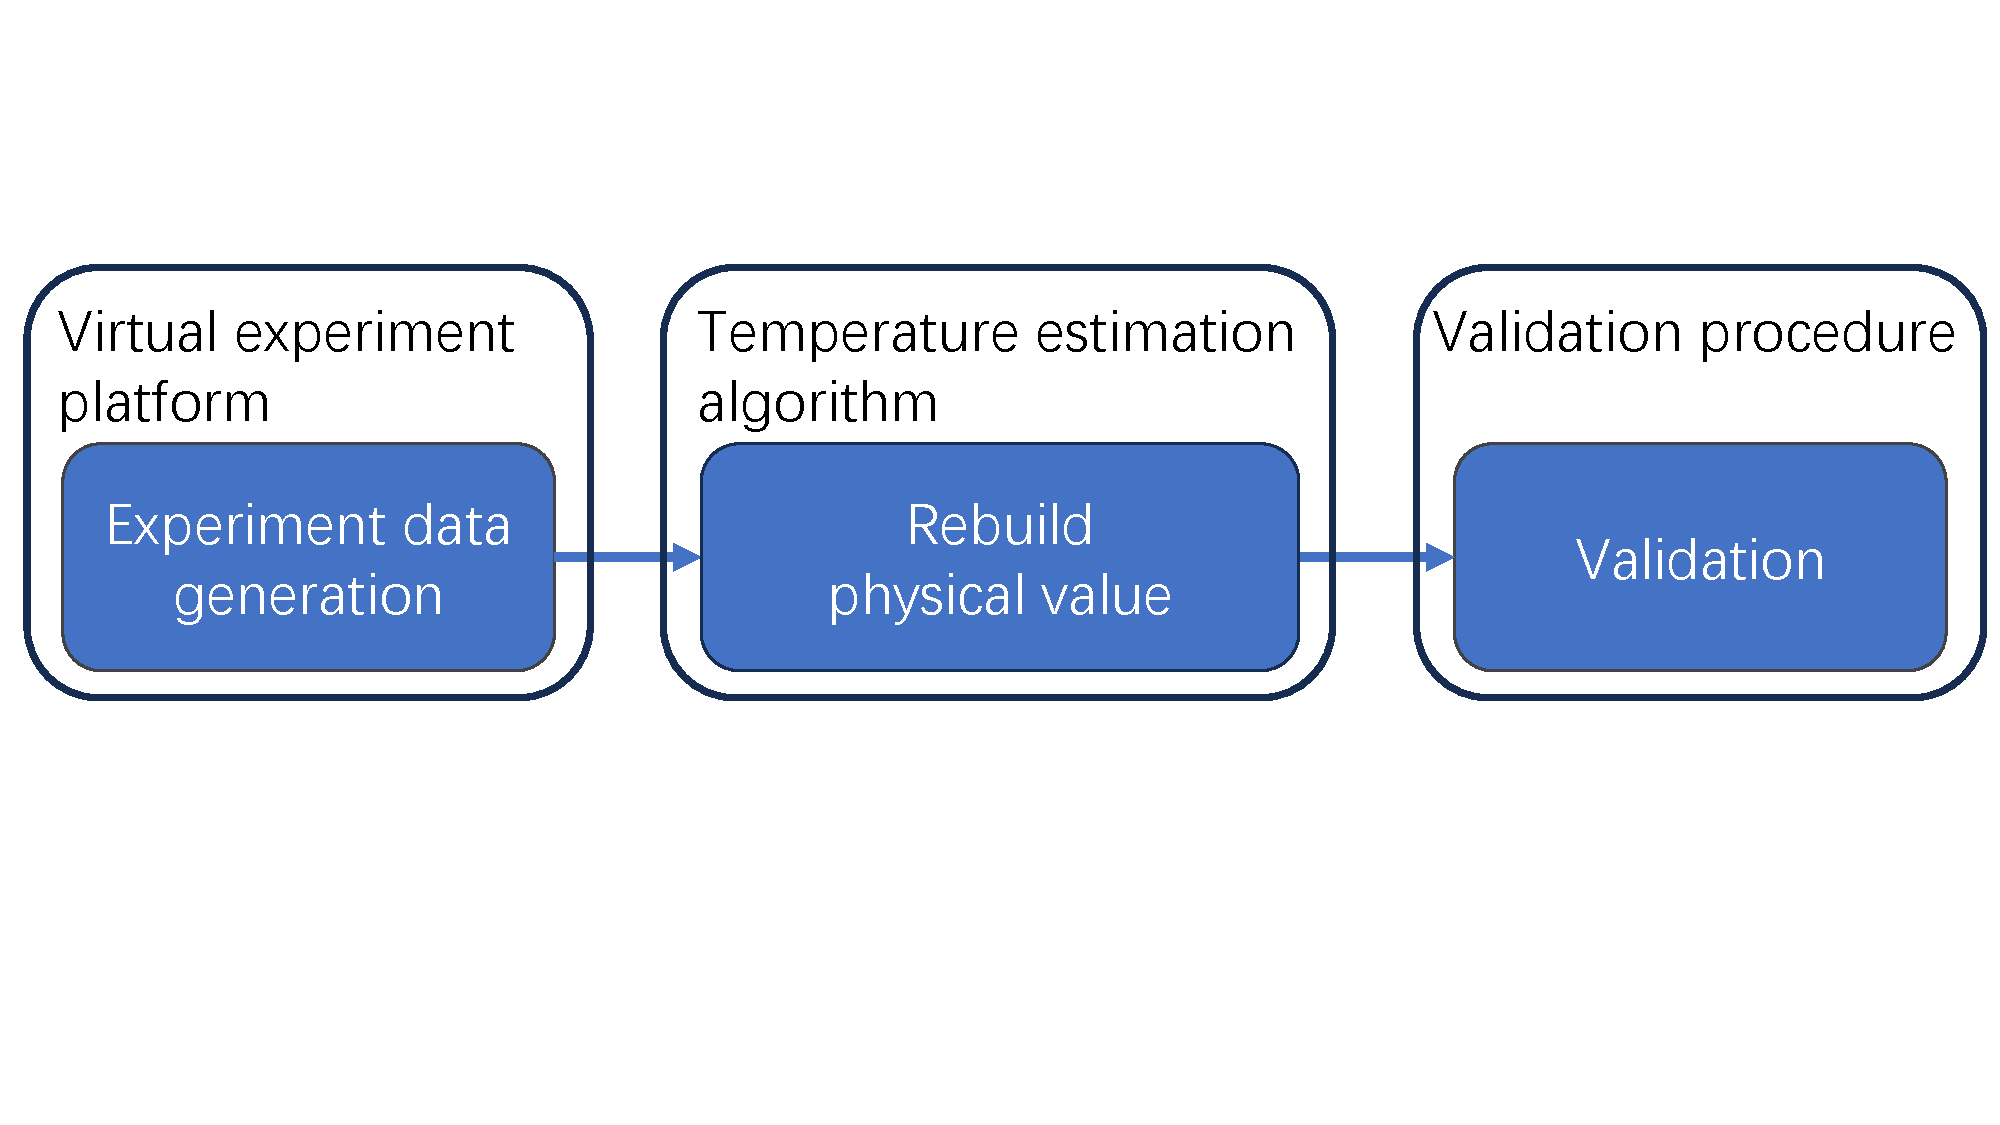
\includegraphics[width=0.90\textwidth]{figures/application_procedure.pdf}
    \caption{Complete procedure from data generation to model validation}
    \label{fig: application_procedure}
\end{figure}


Fig.\ref{fig: application_procedure} shows the procedure of the application.
Firstly, an experiment data set should be generated according to the parameters of the 
hypothetical material. Then, a temperature estimation algorithm is applied to 
estimate the temperature of the hypothetical material. Last, a validation procedure 
is used to check the accuracy and stability of the results of 
temperature estimation algorithm.


As mentioned in previous sections, these functions is implemented in three 
programmes. Namely virtual experiment platform, temperature estimation algorithm
and validation procedure. Similar to conventional experiment methods, these
steps are independent procedures, which means they do not interact with 
each other. 


Accordingly, this chapter will be divided into three sections, which describe 
the implementation and the parameter settings of the virtual experiment platform, 
temperature estimation algorithm and validation procedure.


\section{Experiment data generation}
As the first of the three steps mentioned above, it is crucial to generate 
accurate experimental data correctly. It affects the comparability of the 
virtual experimental platform with real experiments on the one hand, and 
the accuracy of the temperature estimation algorithm on the other. As a 
result, the virtual experimental platform should be able to perform 
calculations for as many hypothetical materials with different properties 
as possible.


In order to be able to obtain image similar to image from
real camera, the area that the virtual camera is able to capture is 
set to a 50*50 pixel picture. Fig.\ref{fig: camera} shows the image obtained 
from real experiment and virtual experiment platform. The major difference between 
these two images is the coloring. In real experiment, the raw image was saved 
as a .tiff file, which obtain the spectral intensity received by the specific 
channel. Then, the intensity is expressed as brightness of the pixel in the display of 
the image. This results in the experiment data that is not intuitive and 
requires specialised software to open these data.


As a result, there are a number of optimisations that have been applied 
in this virtual experiment platform. Firstly, the raw digital value 
of the received spectral intensity was saved in an .xlsx file, which 
simplifies the reading of the data as well as the conversion. In 
addition, a .jpg image of each channel similar to the real experiment data is also 
saved. Different from the real experiment data, colours are used here to 
indicate the value of the spectral intensity. This improves the 
readability of the experiment data.


\begin{figure}[htbp]
    \centering
    \begin{subfigure}{0.45\textwidth}
        \centering
        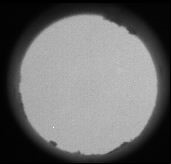
\includegraphics[height=5cm]{figures/real_camera_1075.JPG}
        \caption{Real experiment data  (channel 1)}
        \label{fig: real_camera}
    \end{subfigure}
    % \hfill
    \begin{subfigure}{0.45\textwidth}
        \centering
        
\includegraphics[height=5cm]{figures/virtual_camera_1098.jpg}
        \caption{Virtual experiment data (channel 1)}
        \label{fig: virtual_camera}
    \end{subfigure}
    \caption{Comparison between real experiment data at $1300K$ (a)
    and virtual experiment data at $1098K$ (b)
    }
    \label{fig: camera}
\end{figure}


Thus, the observation area is obtained by initialization of the the virtual 
experiment platform. Temperature field, emissivity model of the hypothetical 
material and the integration method are the parameters to be defined as the next
step.


\subsection{Temperature field}%
As mentioned in previous sections, temperature is one of the most important parameters 
in the virtual experiment platform. In order to obtain results similar to real 
experiments, a temperature field exists in the observation area. For the purpose of 
simplifying the calculation process, this temperature field consists of two main 
regions, a background region at the edge of the observation area, 
where the temperature is uniformly set to 1000K, and an internal high temperature 
region, where the temperature follows a predefined distribution.


\begin{figure}[htbp]
    \centering
    \begin{subfigure}{0.08\textwidth}
        \centering
        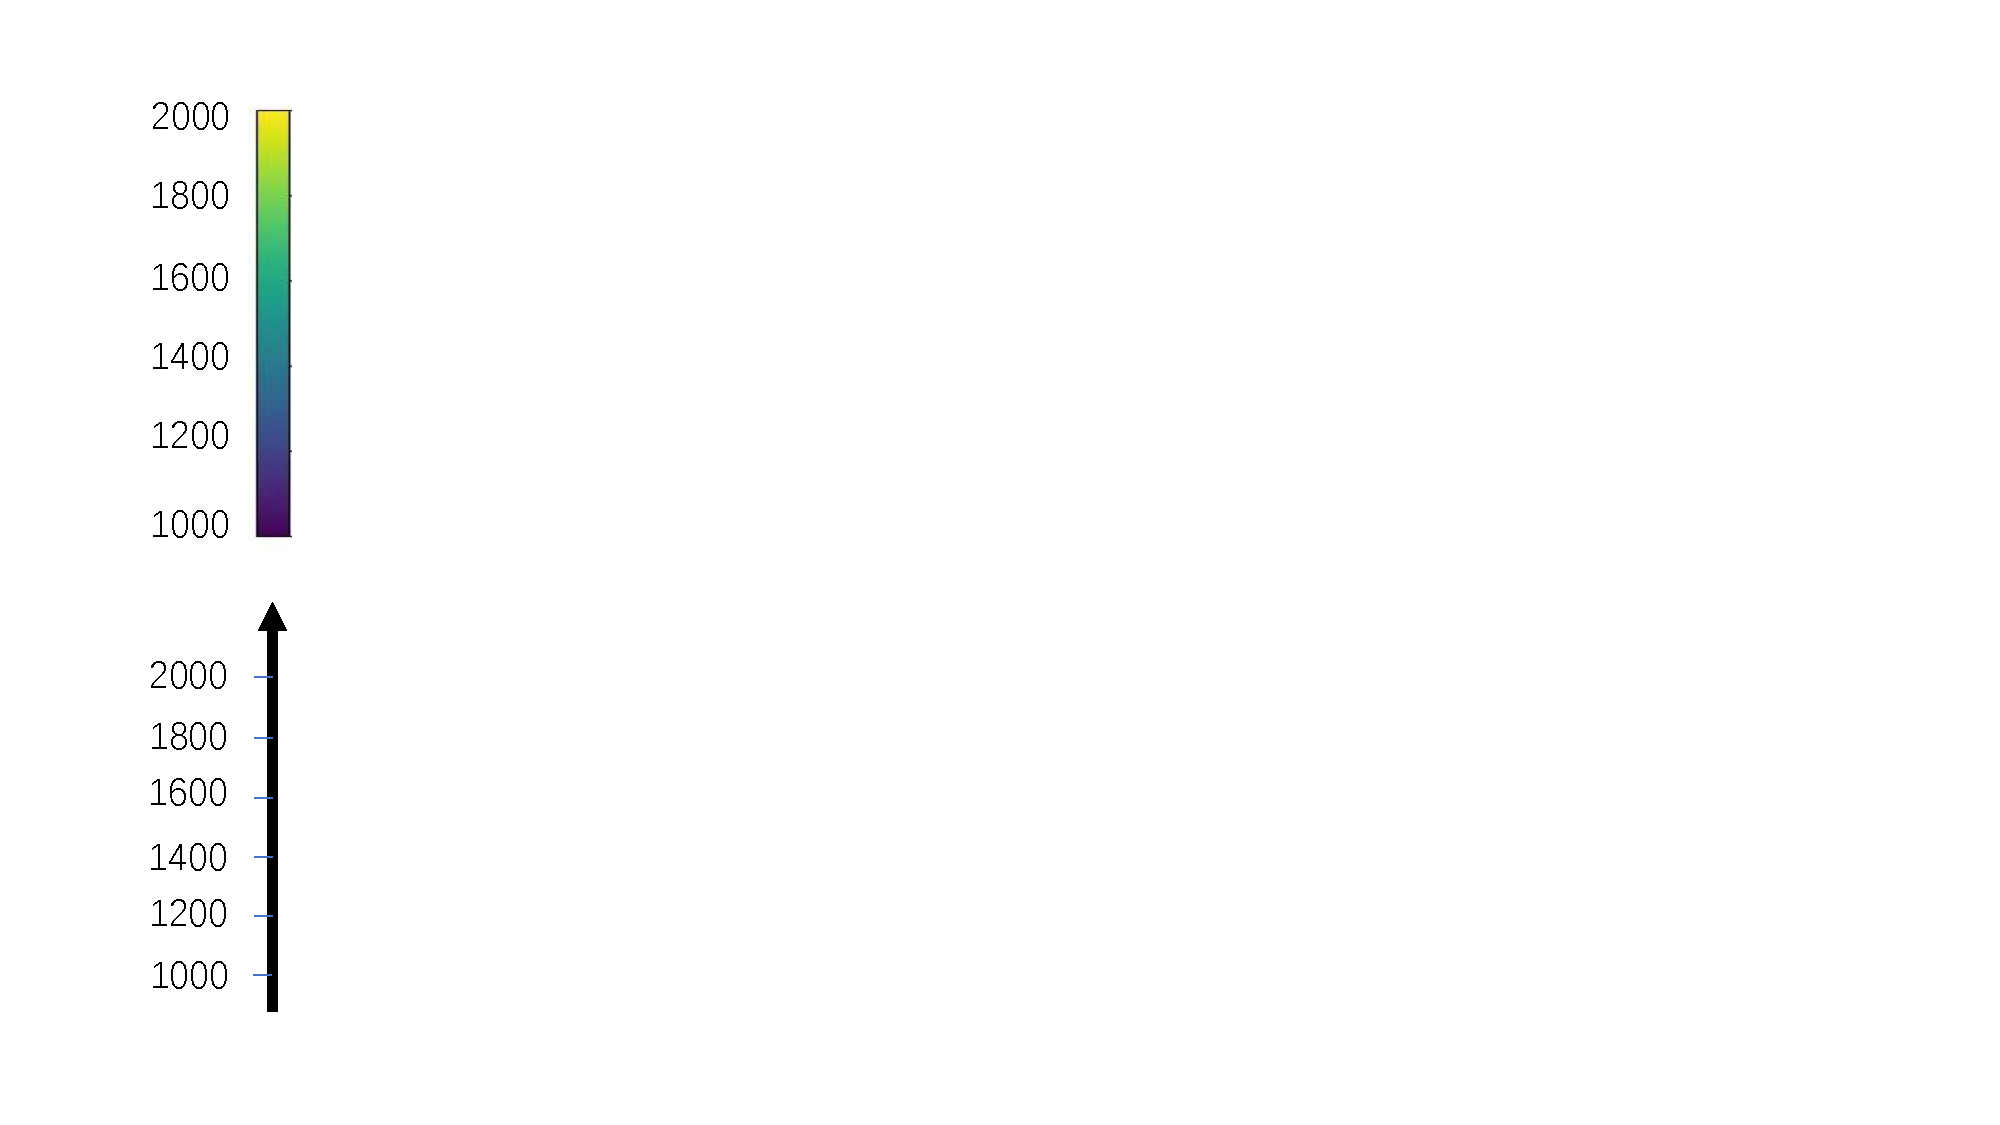
\includegraphics[height=9cm]{figures/temp_distribution_colorbar.pdf}
        \caption*{}        
    \end{subfigure}
    \begin{subfigure}{0.3\textwidth}
        \centering
        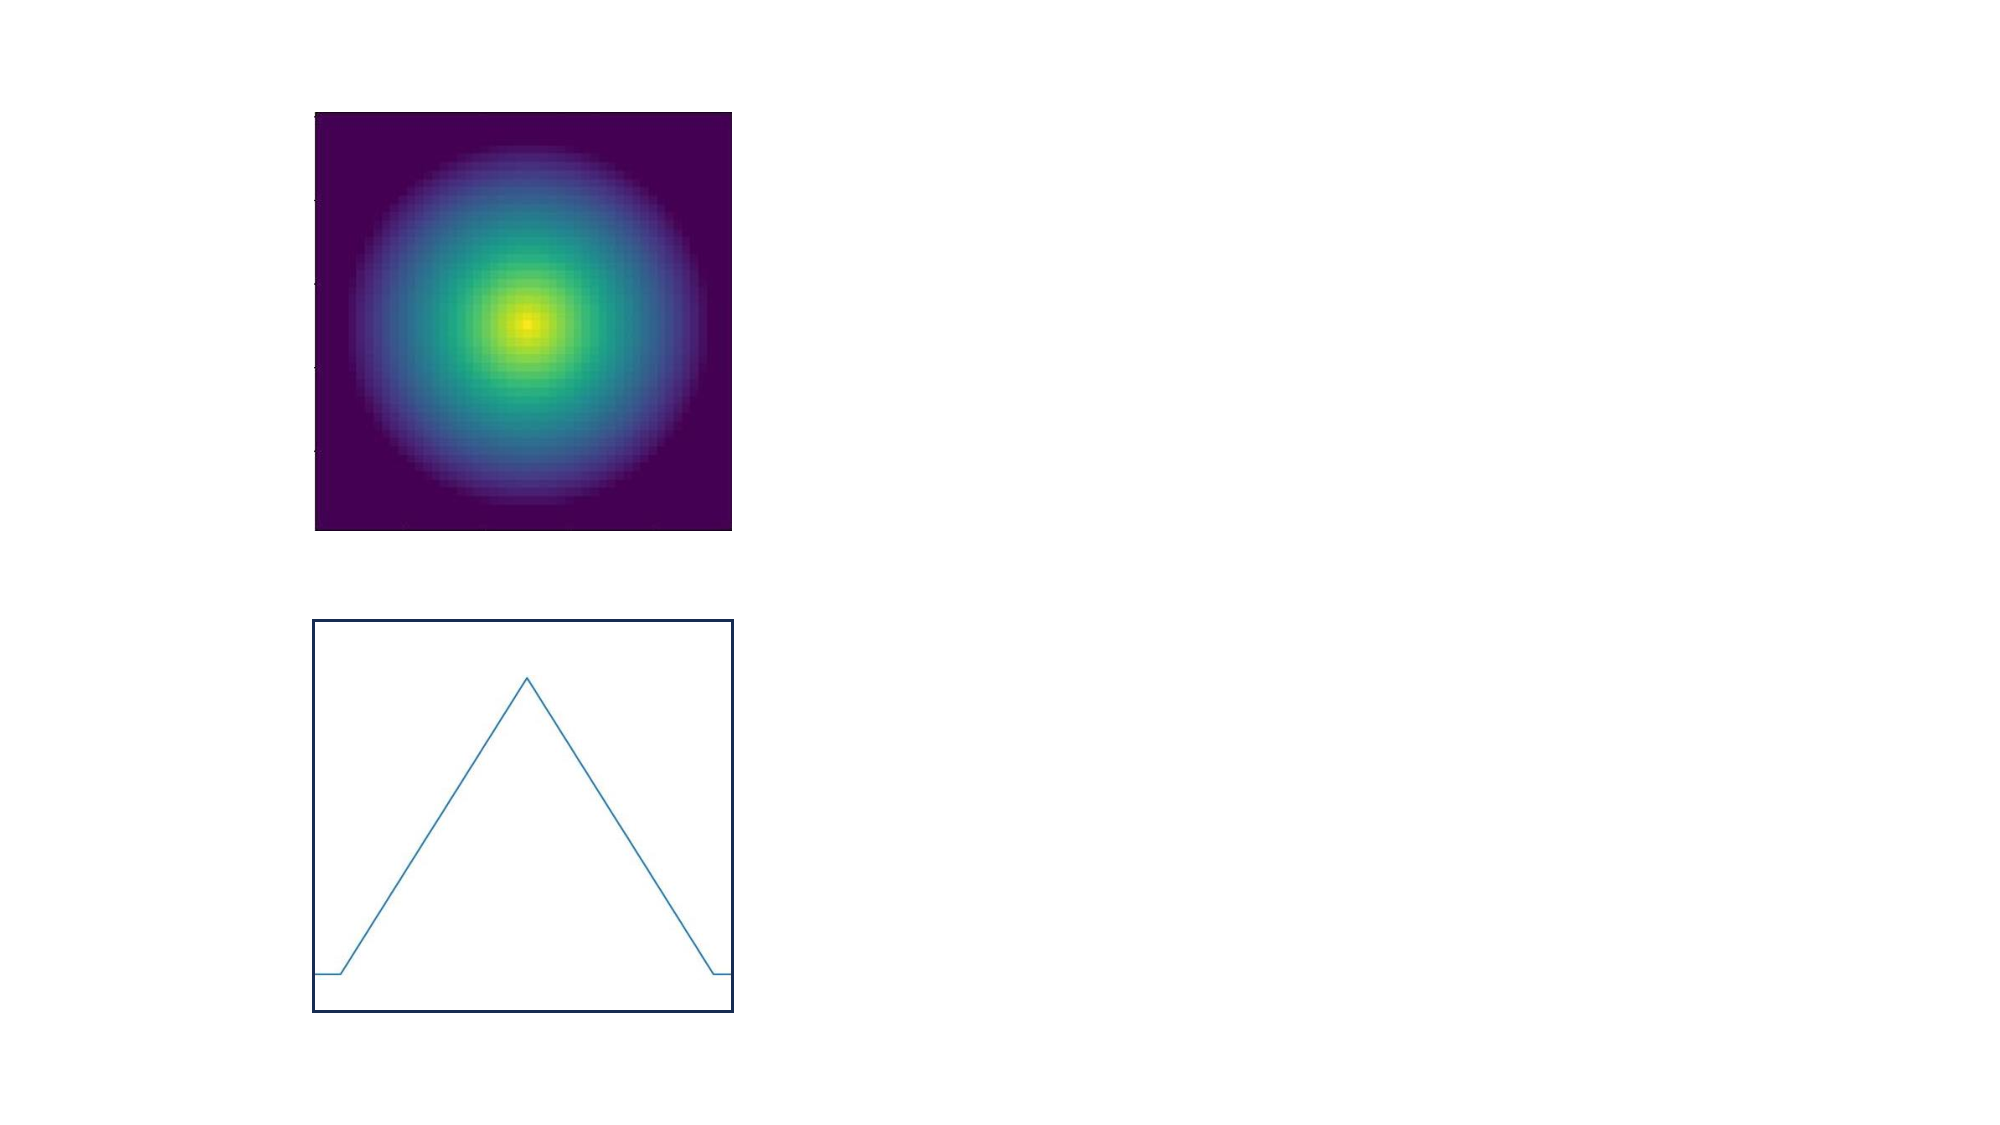
\includegraphics[height=9cm]{figures/temp_distribution_a.pdf}
        \caption{Linear}
        \label{fig: linear_distribution}        
    \end{subfigure}
    \begin{subfigure}{0.3\textwidth}
        \centering
        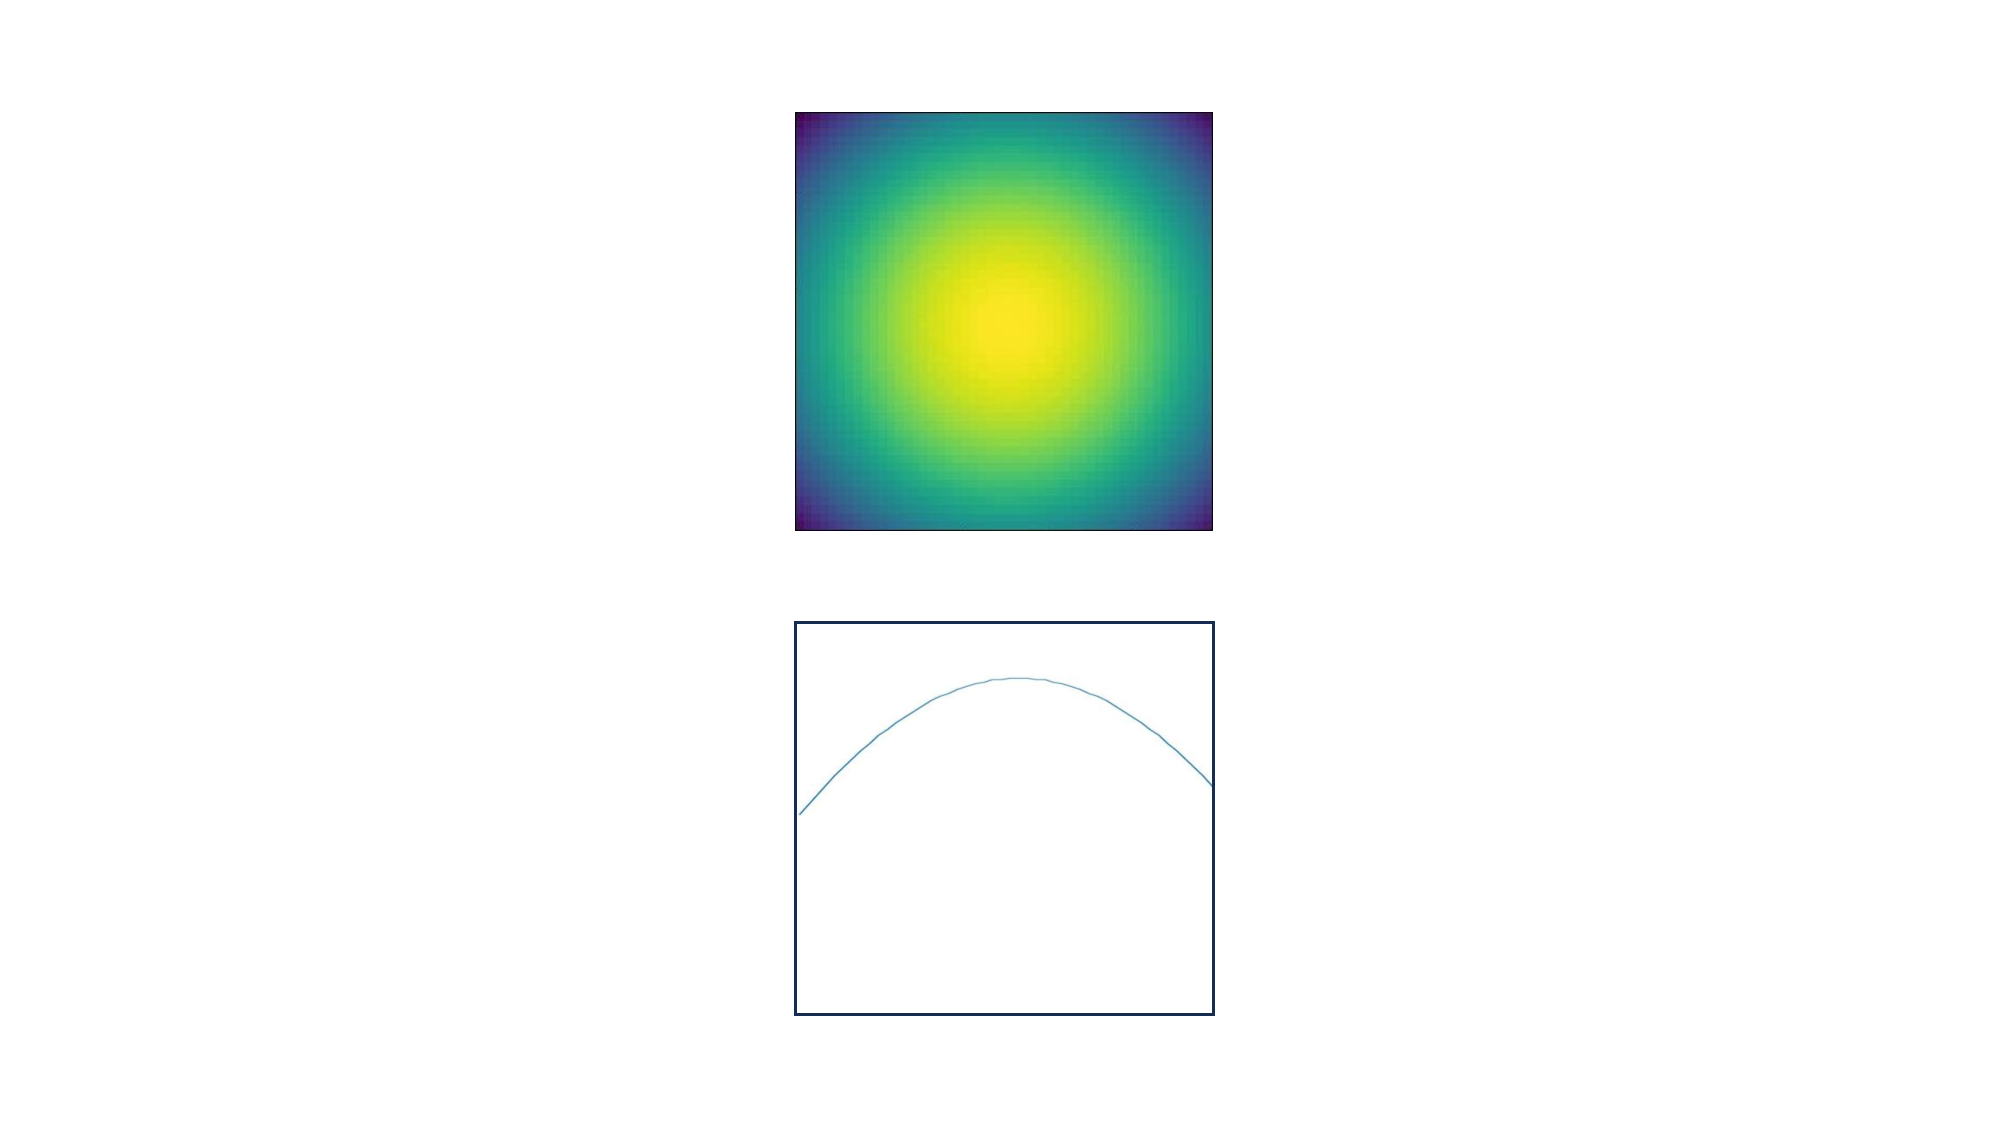
\includegraphics[height=9cm]{figures/temp_distribution_b.pdf}
        \caption{Gaussian}
        \label{fig: gaussian_distribution}        
    \end{subfigure}
    \begin{subfigure}{0.3\textwidth}
        \centering
        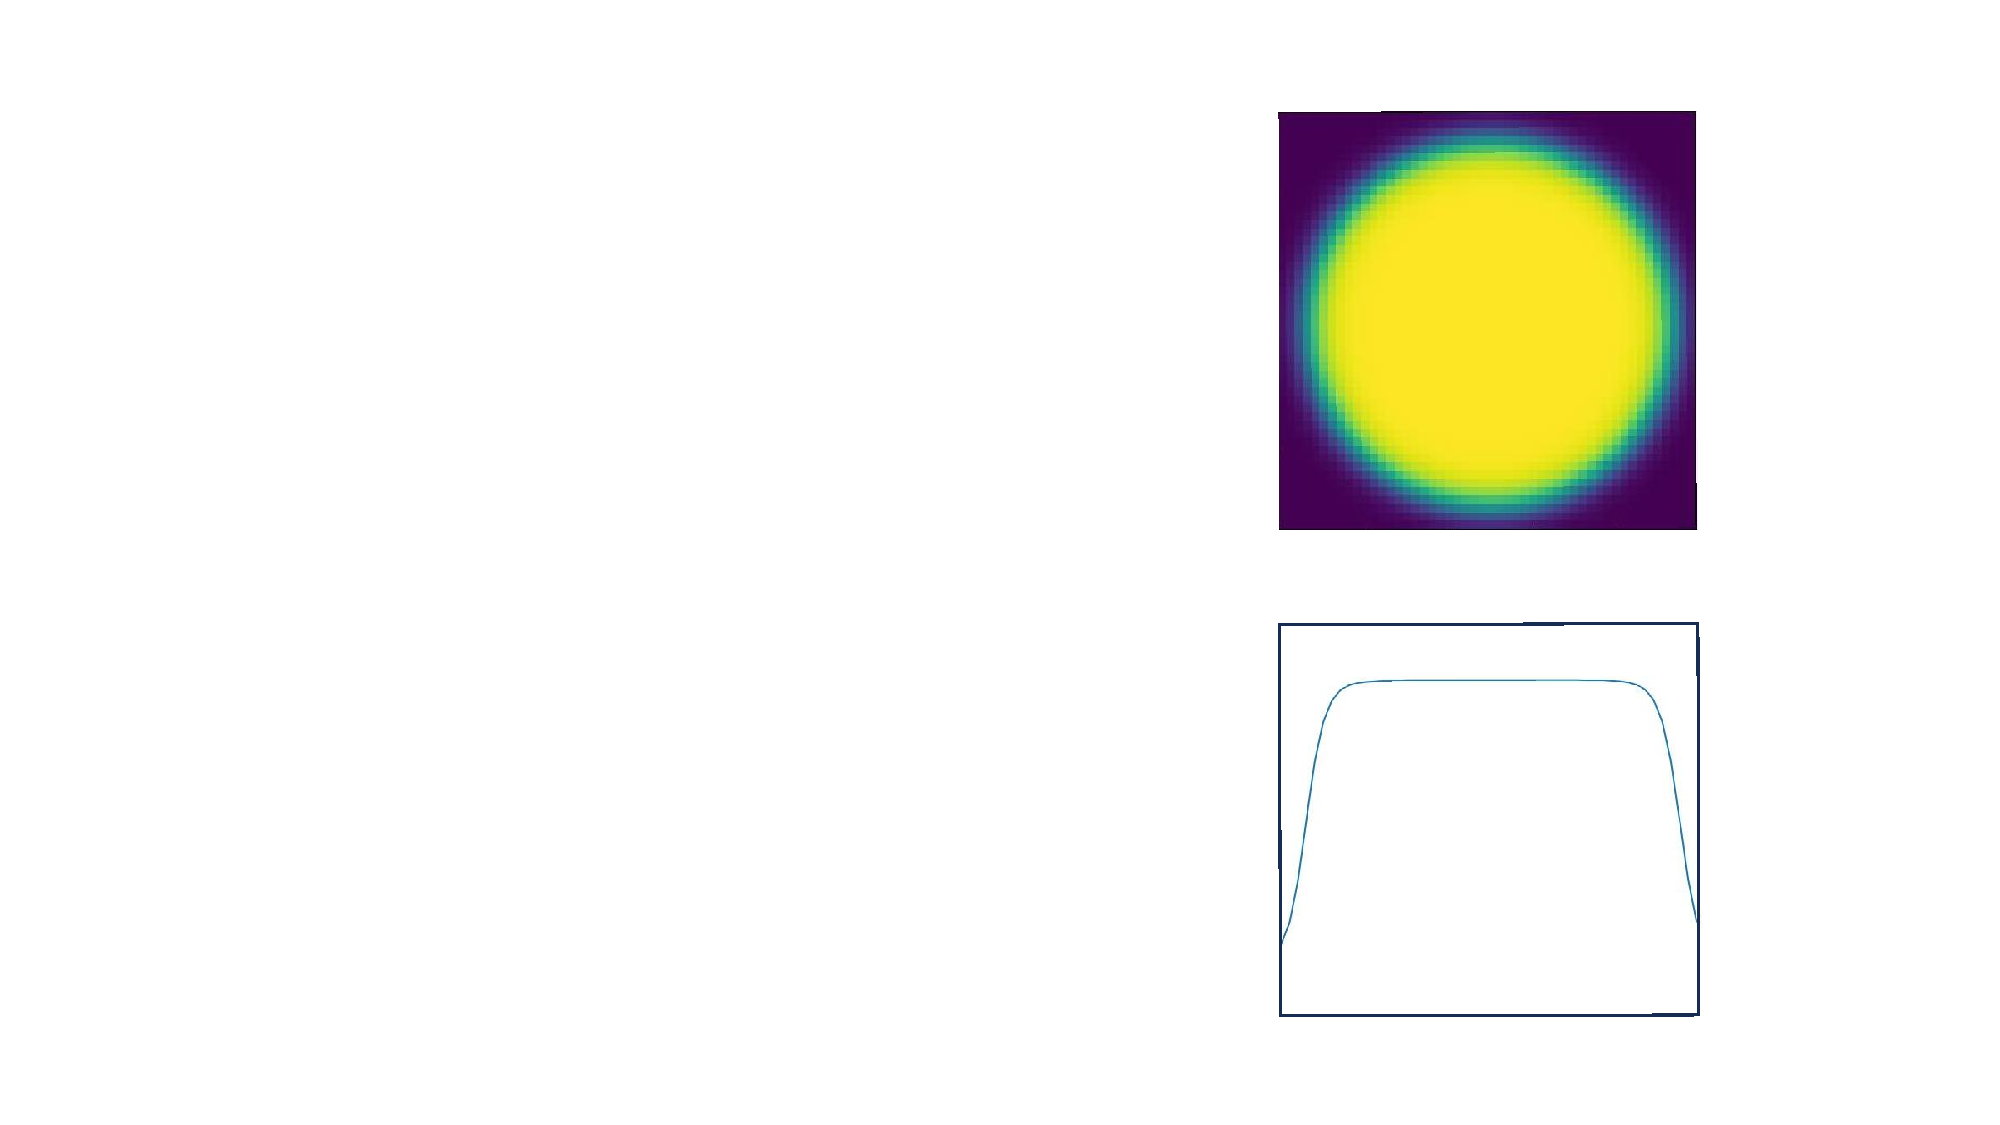
\includegraphics[height=9cm]{figures/temp_distribution_c.pdf}
        \caption{Sigmoid}
        \label{fig: sigmoid_distribution}        
    \end{subfigure}
    \caption{Temperature field of 3 different temperature distribution and the 
    temperature profile in the middle line of the observation area. (\subref{fig: linear_distribution}): 
    Linear distribution. (\subref{fig: gaussian_distribution}): Gaussian distribution. 
    (\subref{fig: sigmoid_distribution}): sigmoid distribution}
    \label{fig: temperature_profile}
\end{figure}


Fig.\ref{fig: temperature_profile} shows three different temperature distribution 
which are able to be generated by the virtual experiment platform. Namely linear 
distribution, gaussian distribution and sigmoid distribution. In order to simplify 
the visualization process, all temperature fields are generated based on the center 
point of the observation area. As the temperature of each point is calculated 
based on the normalized distance $d_{rel}$ or absolute distance ${d_{abs}}$ to the center point of the observation area.


Linear distribution means that the temperature increases linearly from the back ground 
area to the center point of the observation area. The details can be found in 
Eq.\ref{eq: linear_distribution}. This distribution has the potential to 
demonstrate the spectral radiation behavior of the hypothetical material in 
different temperature. 


\begin{equation}
    t = t_{center} + (t_{background} - t_{center}) \cdot d_{rel}
    \label{eq: linear_distribution}
\end{equation}


Gaussian distribution is also called normal distribution. In this distribution 
type, the temperature field in observation area obeys gaussian distribution described 
in Eq.\ref{eq: gaussian_distribution}. With the temperature of the center 
point in observation area equals the defined center temperature. Due to energy input 
of the system and heat transfer in metal powder, this temperature distribution 
is more likely to simulate the real situation in experiment.

\begin{equation}
    t = t_{center} + (t_{background} - t_{center}) \cdot \exp {\left(-\frac{d_{abs}}{2 \cdot \sigma^2}\right)}
    \label{eq: gaussian_distribution}
\end{equation}


Different to the temperature field mentioned before, the temperature in the center region 
of observation area remains constant. The mathematical expression can be found in 
Eq.\ref{eq: sigmoid_distribution}:

\begin{equation}
    t = t_{center} + (t_{background} - t_{center}) \cdot \sigmoid\left( \left(\frac{d_{abs}^2}{r_{set}^2} + 1\right)\cdot 1000\right)
    \label{eq: sigmoid_distribution}
\end{equation}


With sigmoid function can be found in Eq.\ref{eq: sigmoid_function}:

\begin{equation}
    \sigmoid(x) = \left(1 + \exp\left(-\frac{x}{100}\right)\right)
    \label{eq: sigmoid_function}
\end{equation}


Sigmoid function gaves the opportunity to perform the temperature estimation algorithm 
in a stable temperature. Thus, the potential to investigate the consistency of the 
temperature estimation algorithm and performance of the noise cancellation program is 
given. 


\subsection{Emissivity model}%
Obtaining temperature field of the hypothetical material, an emissivity model 
is required to calculate the physical value of spectral radiation intensity 
emitted from the hypothetical material.


\begin{figure}[htbp]
    \centering
    \begin{subfigure}{0.3\linewidth}
      \centering
      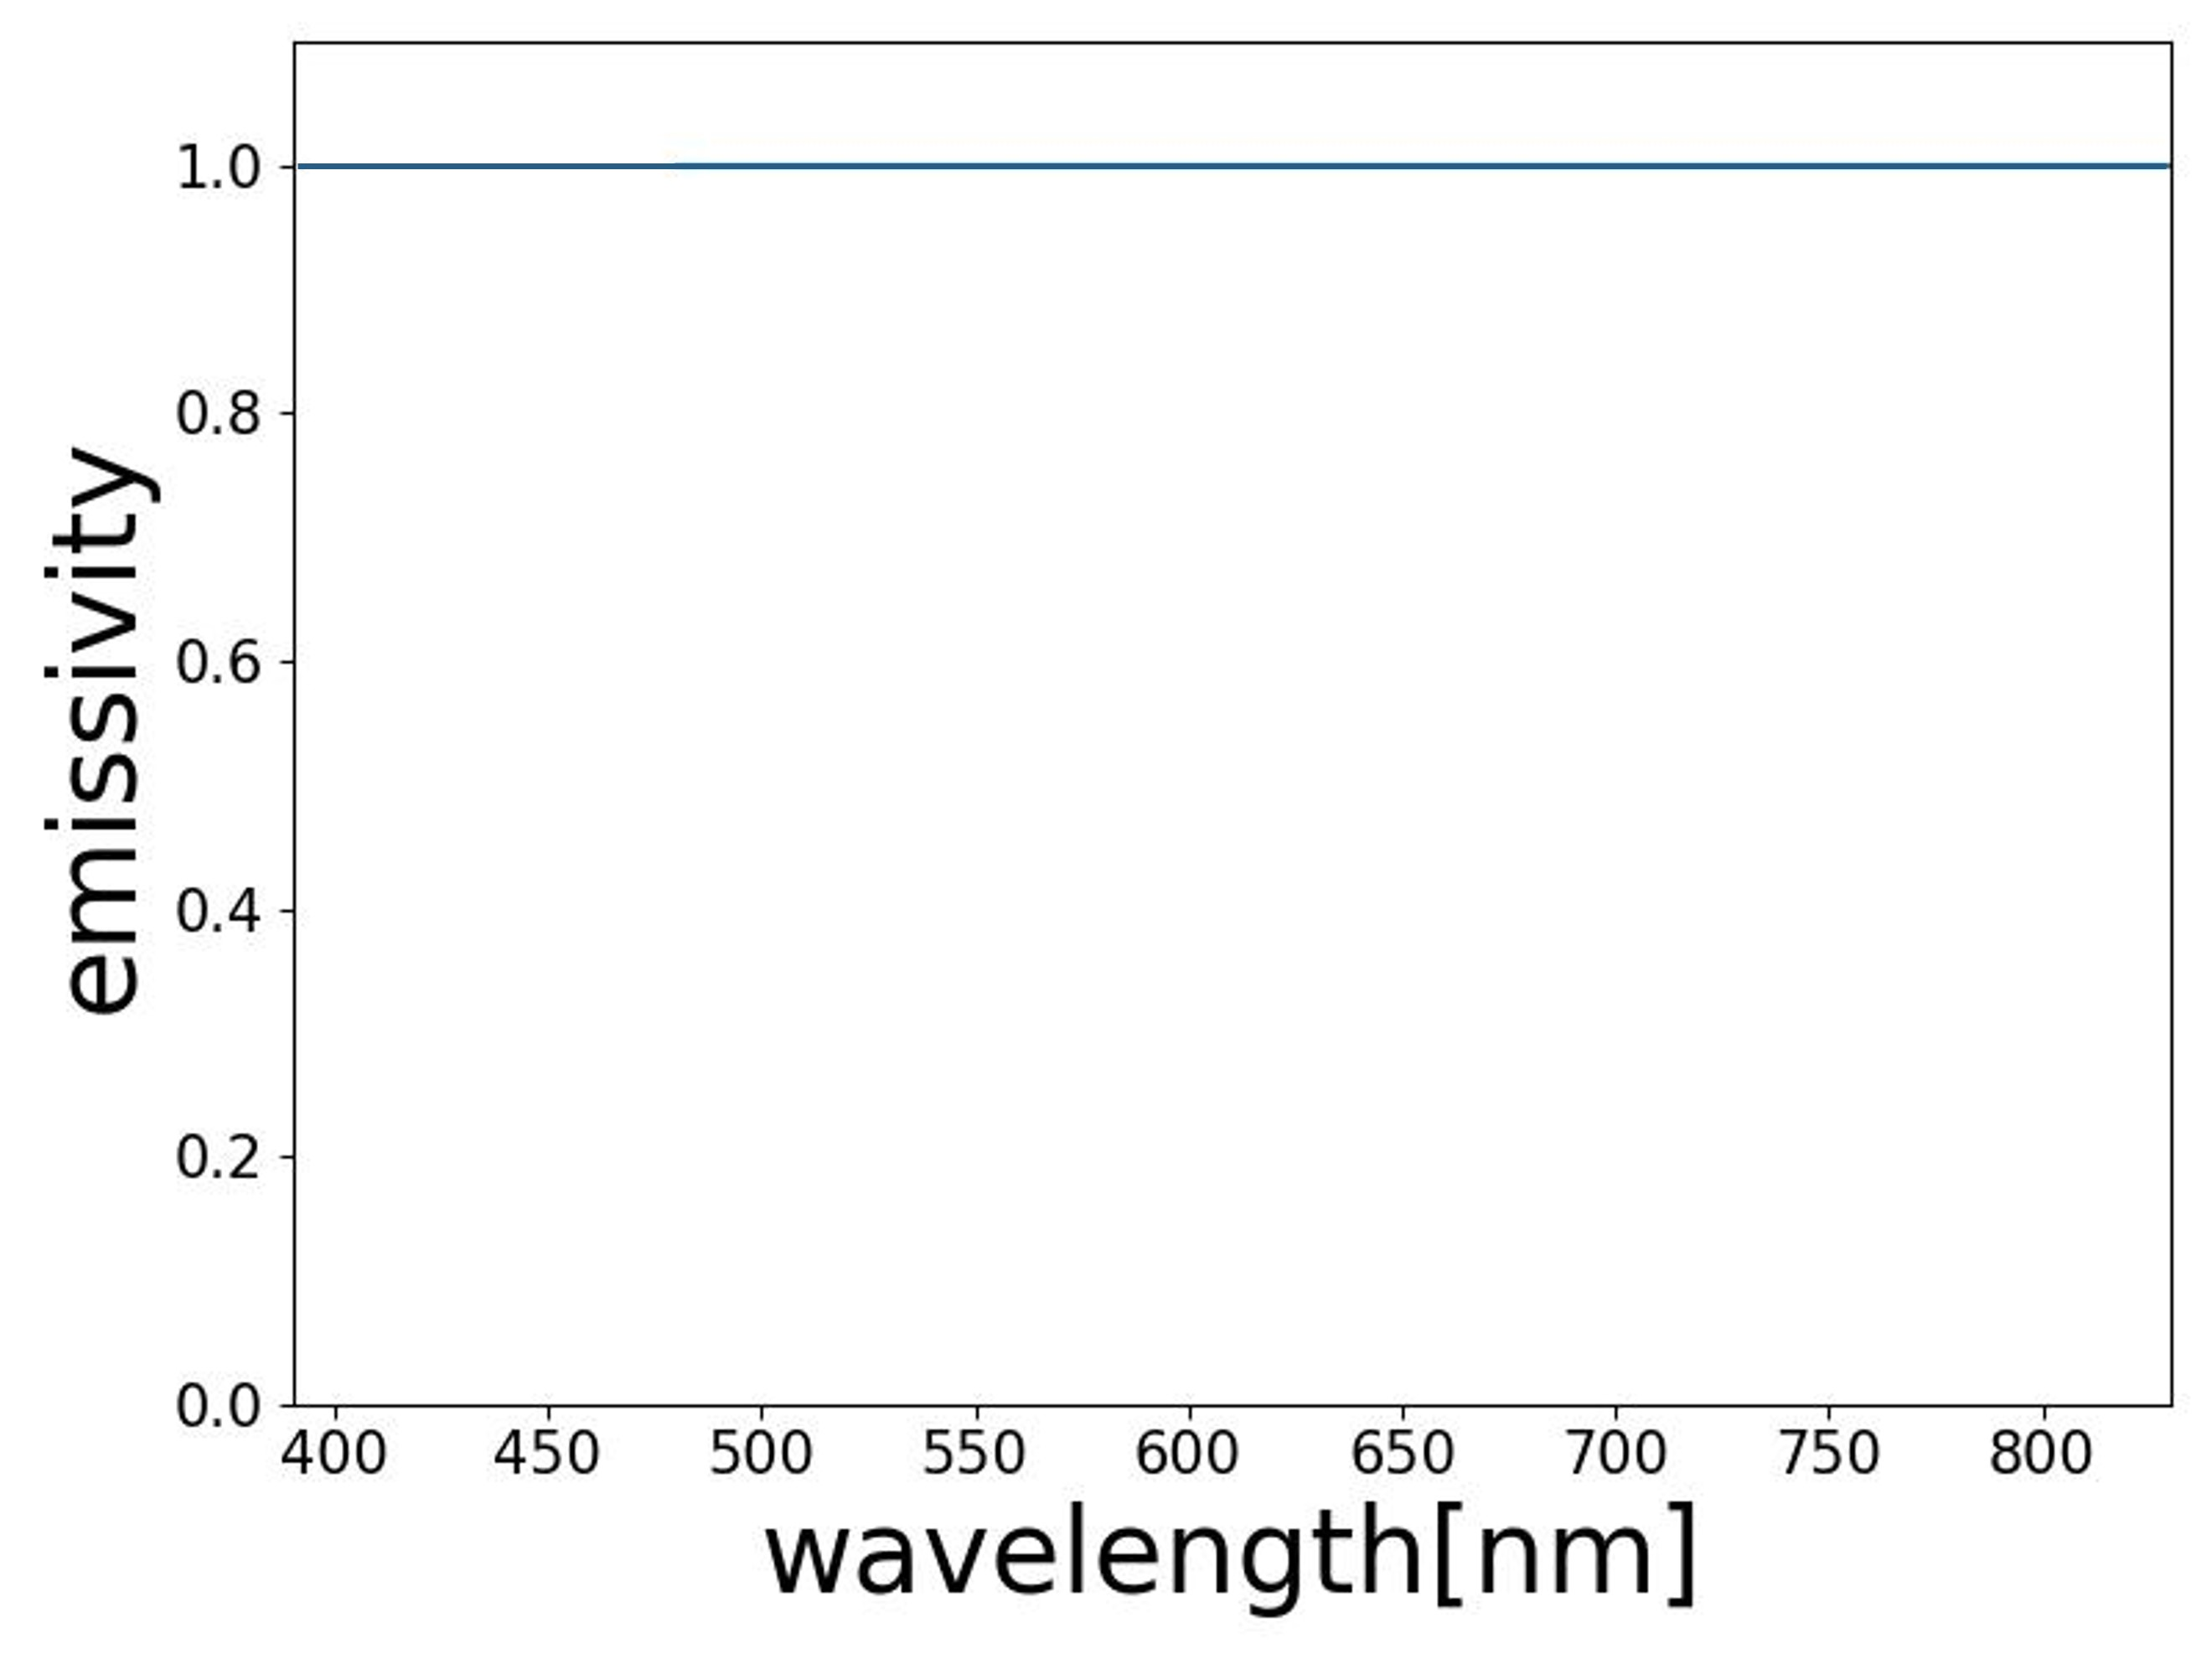
\includegraphics[width=\linewidth]{figures/emissivity_0.jpg}
      \caption{Black body model}
      \label{fig: emi_0}
    \end{subfigure}
    \hfill
    \begin{subfigure}{0.3\linewidth}
      \centering
      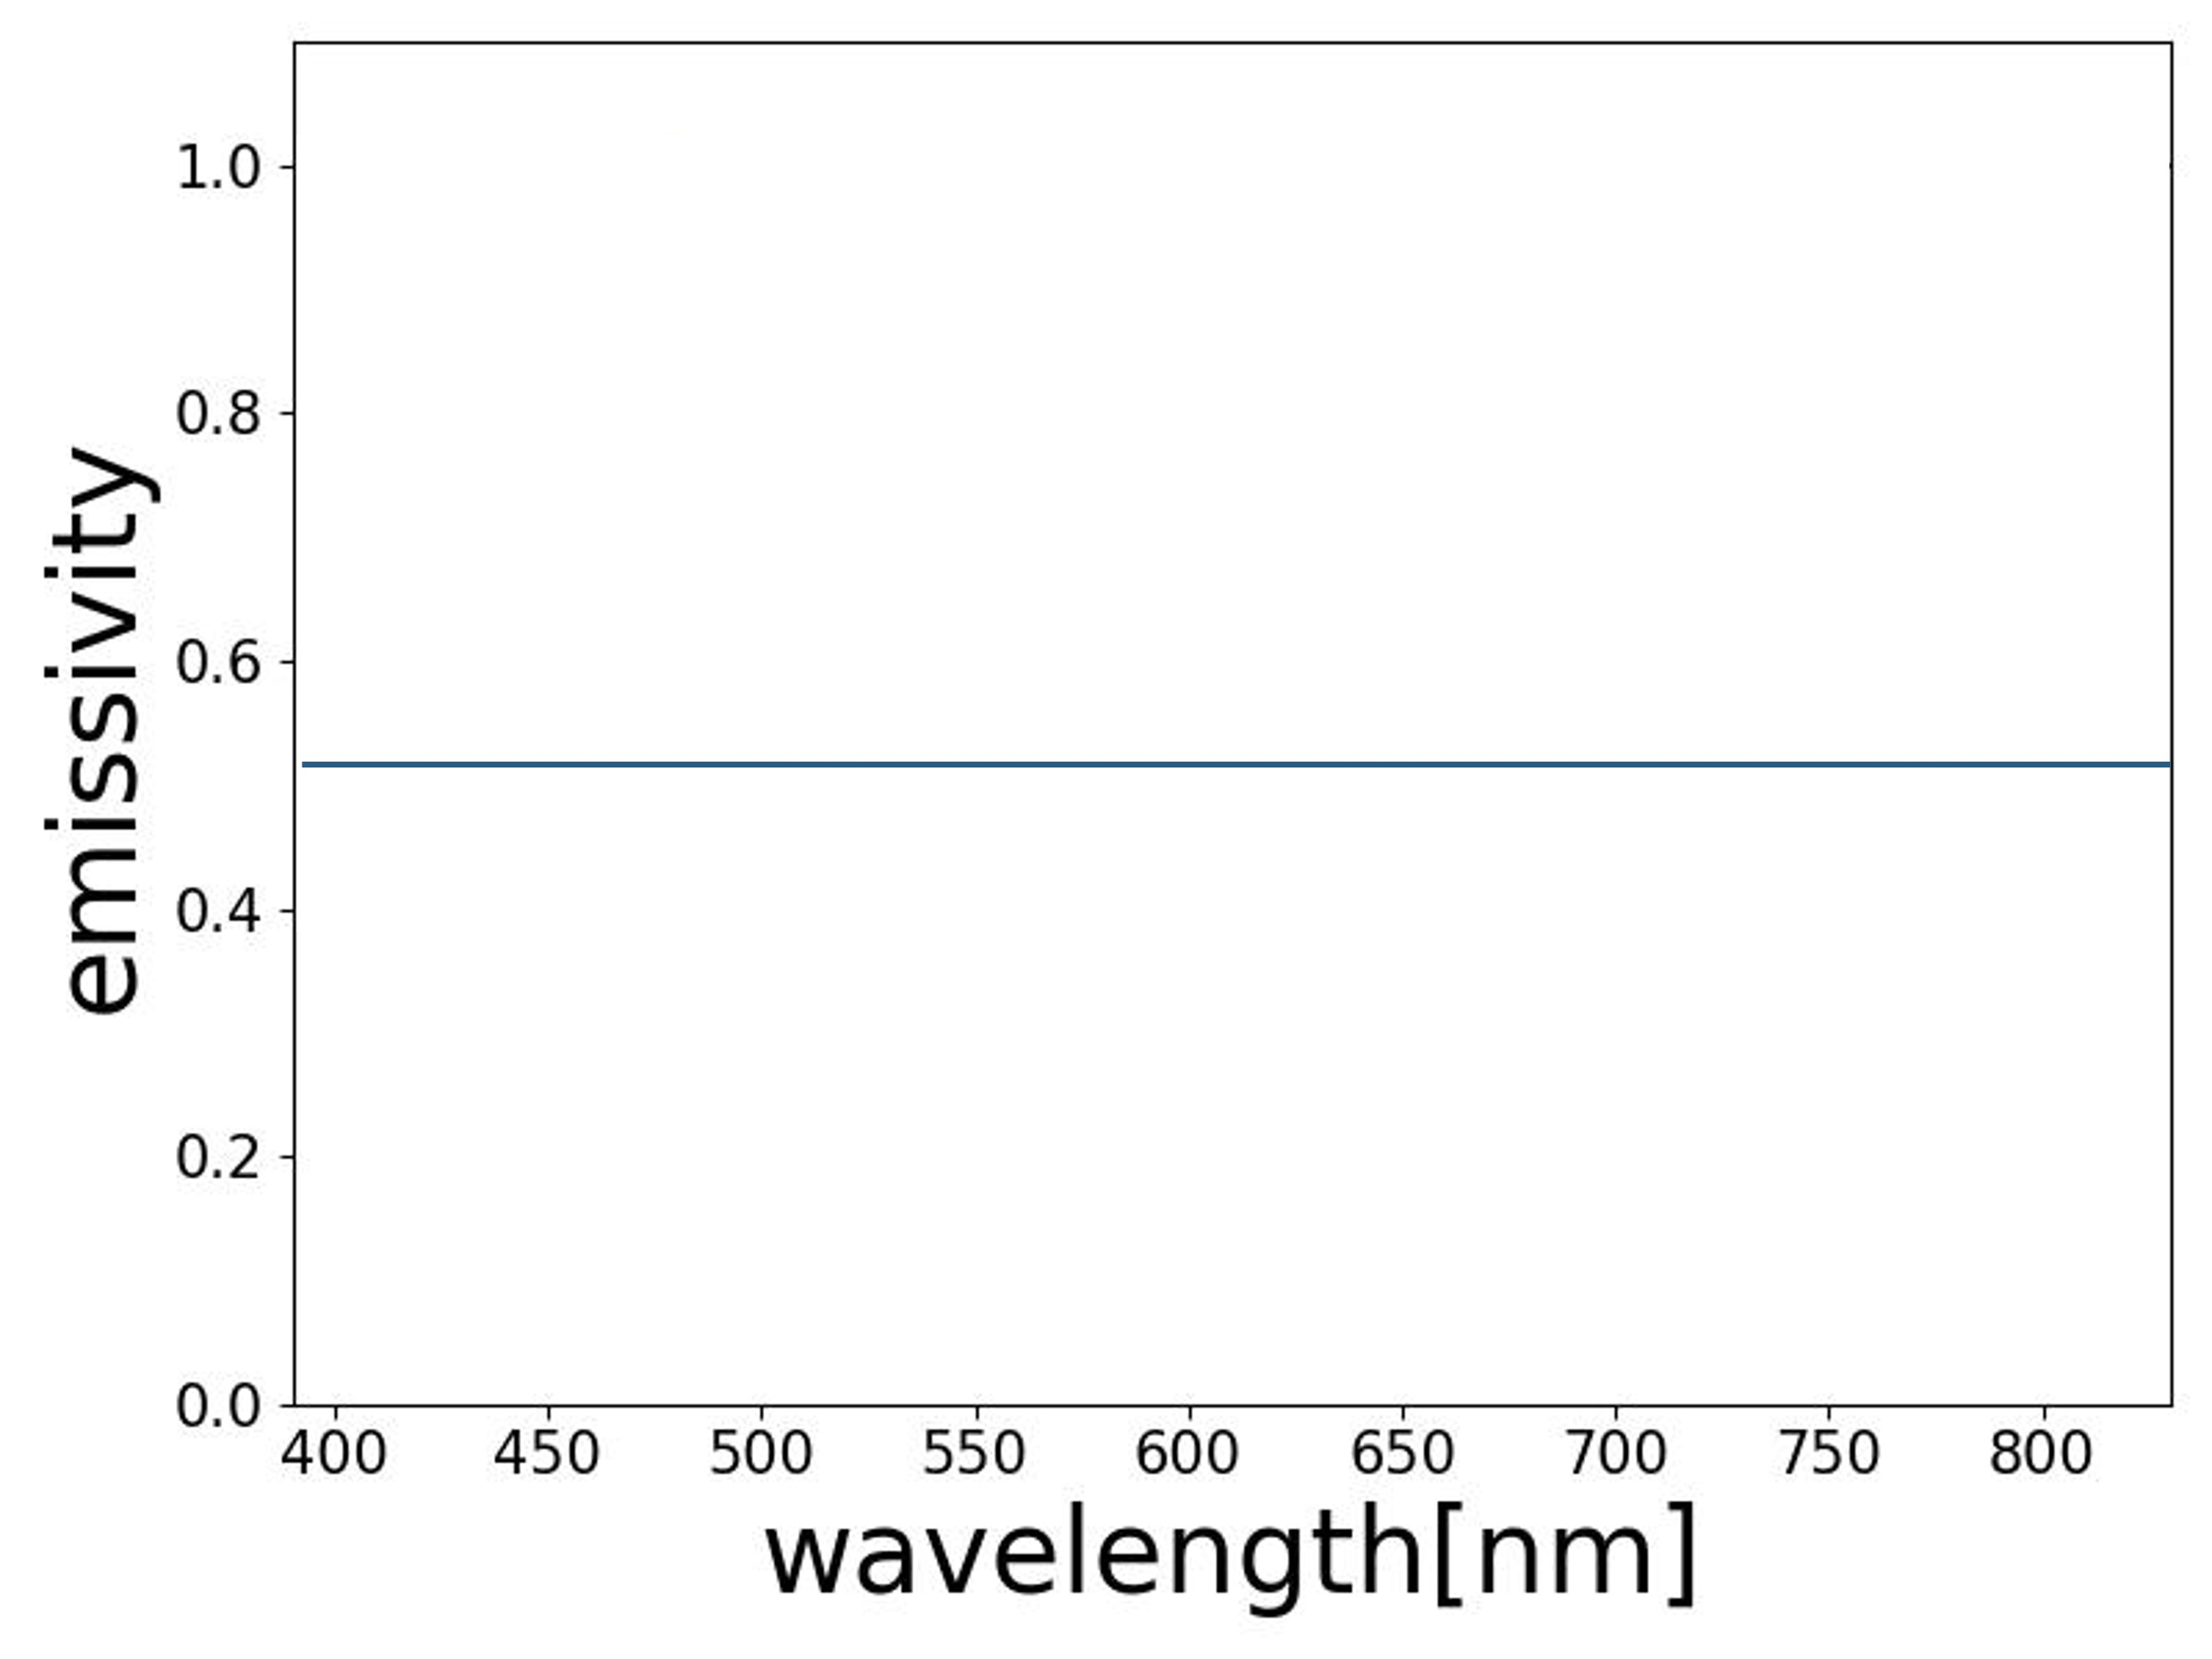
\includegraphics[width=\linewidth]{figures/emissivity_1.jpg}
      \caption{Gray body model}
      \label{fig: emi_1}
    \end{subfigure}
    \hfill
    \begin{subfigure}{0.3\linewidth}
      \centering
      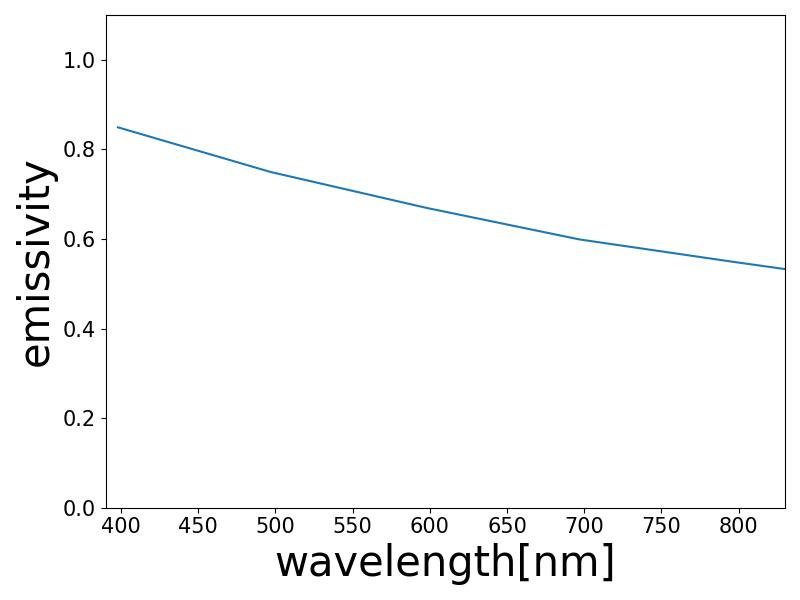
\includegraphics[width=\linewidth]{figures/emissivity_21.jpg}
      \caption{Model 1}
      \label{fig: emi_21}
    \end{subfigure}
    
    \medskip
    
    \begin{subfigure}{0.3\linewidth}
      \centering
      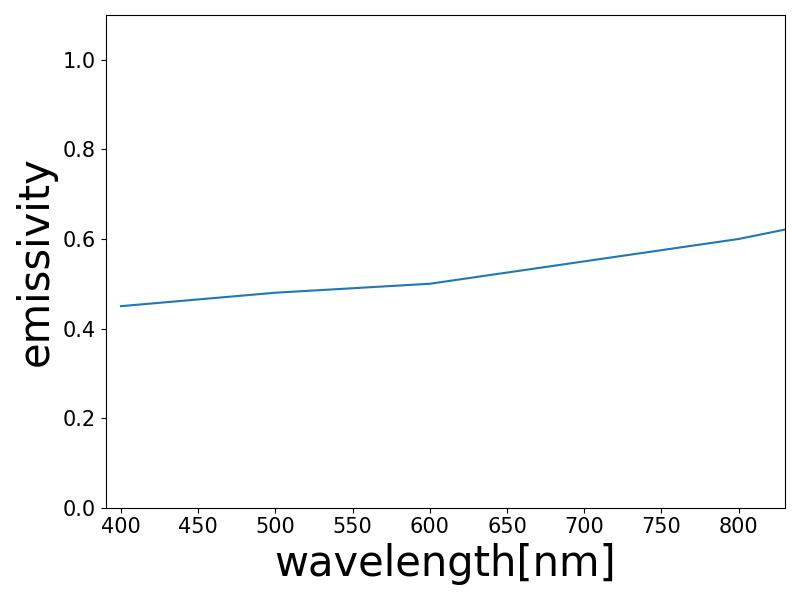
\includegraphics[width=\linewidth]{figures/emissivity_22.jpg}
      \caption{Model 2}
      \label{fig: emi_22}
    \end{subfigure}
    \hfill
    \begin{subfigure}{0.3\linewidth}
      \centering
      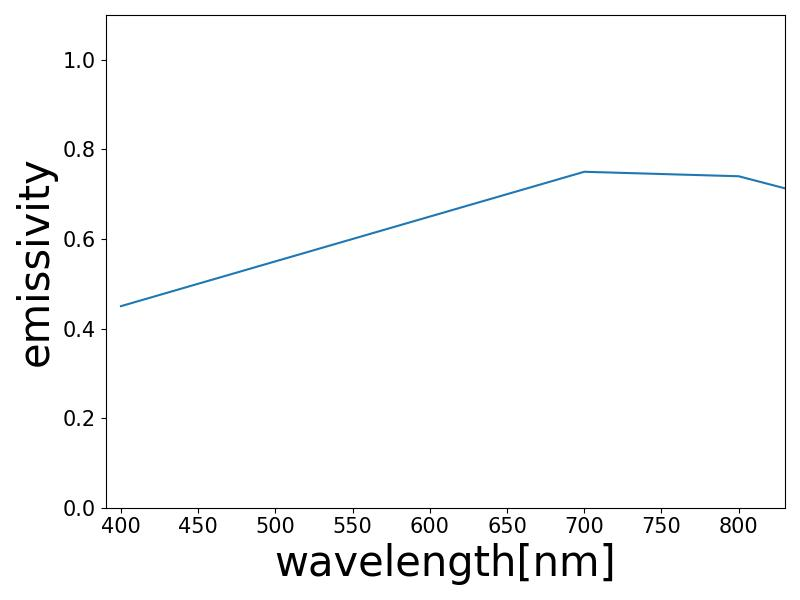
\includegraphics[width=\linewidth]{figures/emissivity_23.jpg}
      \caption{Model 3}
      \label{fig: emi_23}
    \end{subfigure}
    \hfill
    \begin{subfigure}{0.3\linewidth}
      \centering
      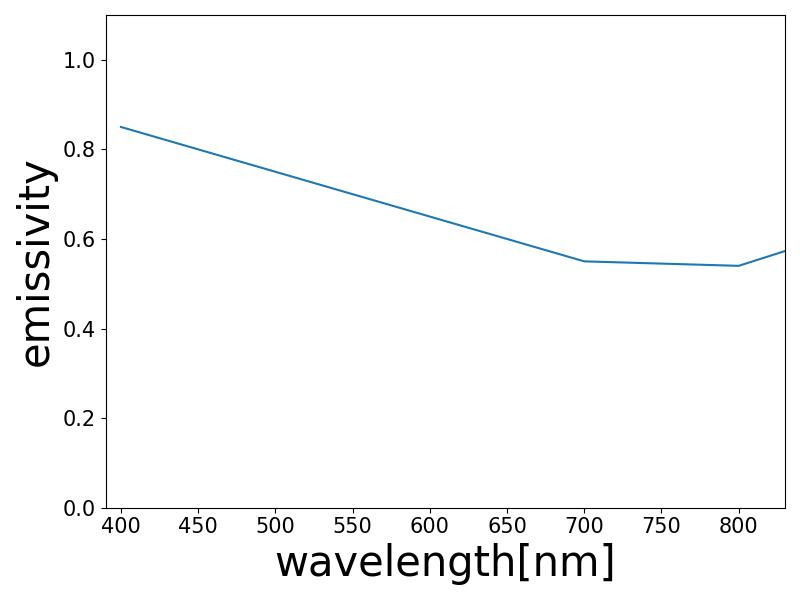
\includegraphics[width=\linewidth]{figures/emissivity_24.jpg}
      \caption{Model 4}
      \label{fig: emi_24}
    \end{subfigure}
    
    \medskip
    
    \begin{subfigure}{0.3\linewidth}
      \centering
      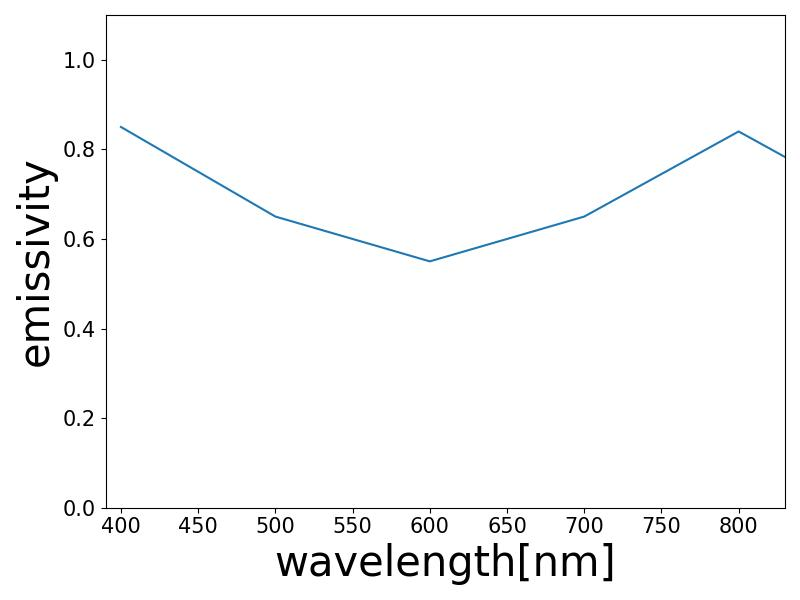
\includegraphics[width=\linewidth]{figures/emissivity_25.jpg}
      \caption{Model 5}
      \label{fig: emi_25}
    \end{subfigure}
    \hfill
    \begin{subfigure}{0.3\linewidth}
      \centering
      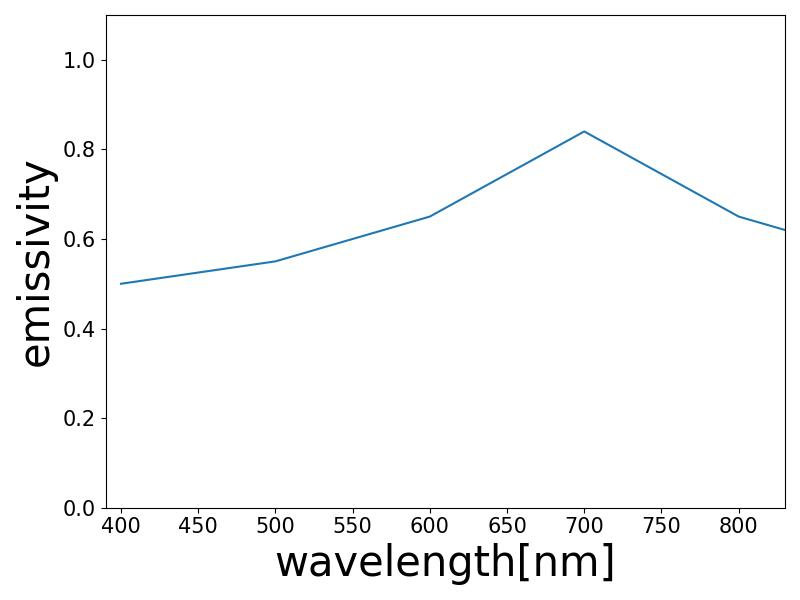
\includegraphics[width=\linewidth]{figures/emissivity_26.jpg}
      \caption{Model 6}
      \label{fig: emi_26}
    \end{subfigure}
    \hfill
    \begin{subfigure}{0.3\linewidth}
      \centering
      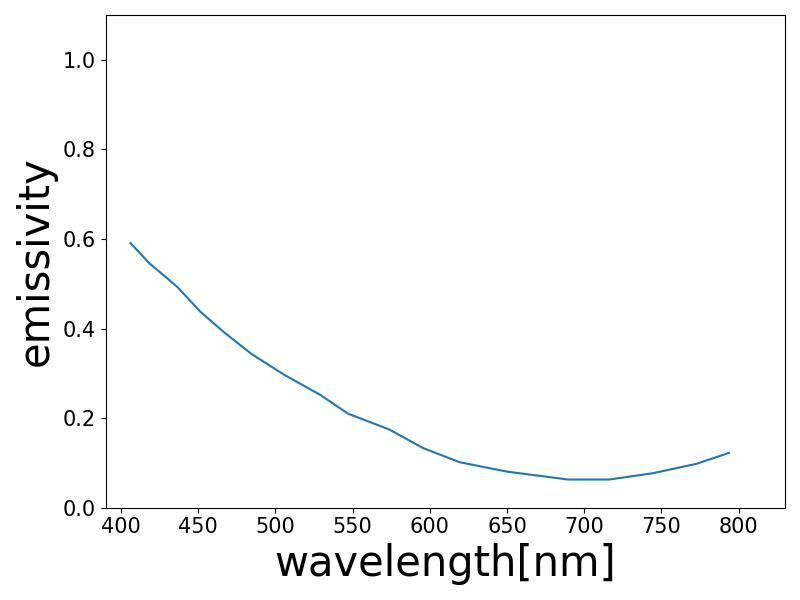
\includegraphics[width=\linewidth]{figures/emissivity_31.jpg}
      \caption{Model 7}
      \label{fig: emi_31}
    \end{subfigure}
    
    \medskip
    
    \begin{subfigure}{0.3\linewidth}
      \centering
      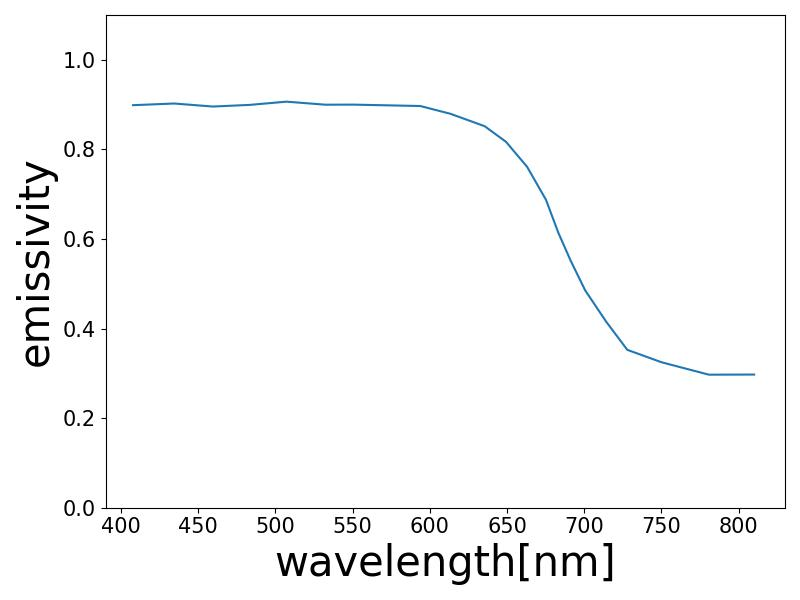
\includegraphics[width=\linewidth]{figures/emissivity_32.jpg}
      \caption{Model 8}
      \label{fig: emi_32}
    \end{subfigure}
    \hfill
    \begin{subfigure}{0.3\linewidth}
      \centering
      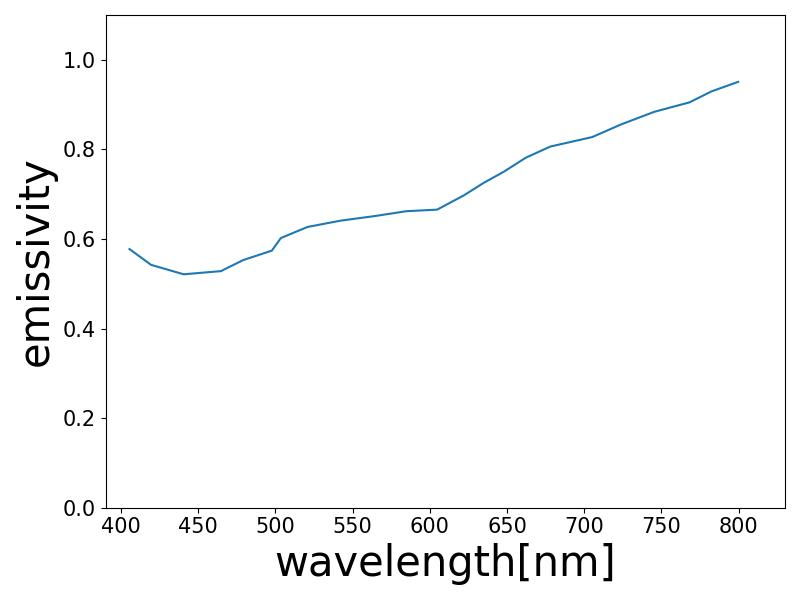
\includegraphics[width=\linewidth]{figures/emissivity_33.jpg}
      \caption{Model 9}
      \label{fig: emi_33}
    \end{subfigure}
    \hfill
    \begin{subfigure}{0.3\linewidth}
      \centering
      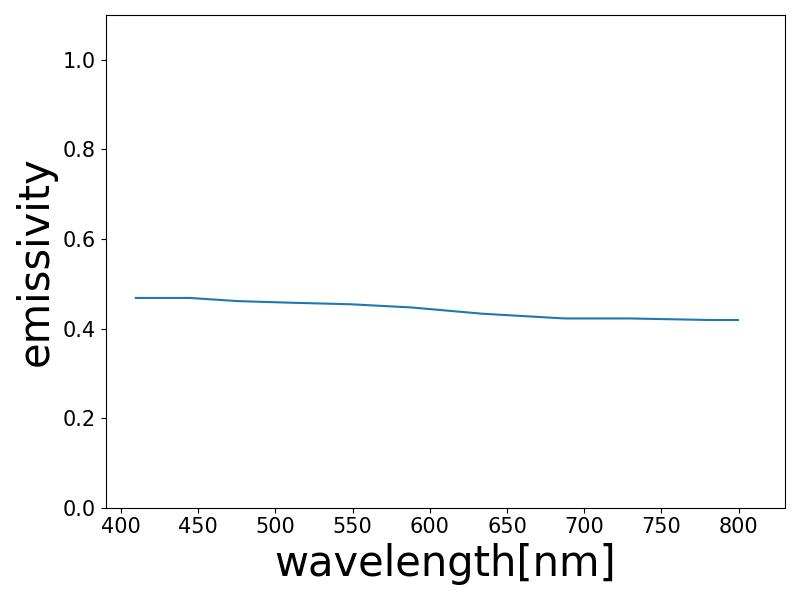
\includegraphics[width=\linewidth]{figures/emissivity_34.jpg}
      \caption{Model 10}
      \label{fig: emi_34}
    \end{subfigure}
    
    \caption{Raw emissivity data used in virtual experiment platform. (\subref{fig: emi_0}), 
    (\subref{fig: emi_1}) are black body and gray body; (\subref{fig: emi_21}) - (\subref{fig: emi_26})
    are hypothetical materials\cite{Wang.2021b}; (\subref{fig: emi_31}) - 
    (\subref{fig: emi_34}) are real materials\cite{Taunay.2020b}.}
    \label{fig: emi_model}
\end{figure}


Since the emissivity of metal powder is wavelength ($\lambda$) and temperature 
($T$) relevant, the emissivity model in this virtual experiment platform is 
formed based on the Eq.\ref{eq: emissivity}. 


\begin{equation}
  \label{eq: emissivity}
  \varepsilon(\lambda, T) = \varepsilon _{raw}(\lambda) \cdot K_T(T)
\end{equation}


The raw emissivity data $\varepsilon_{raw}(\lambda)$ in Fig.\ref{fig: emi_model}
are obtained by Wang et al.\cite{Wang.2021b} and Taunay et 
al.\cite{Taunay.2020b}. These data sets could be used to simulate the 
radiation behavior of various hypothetical materials.


After obtaining the raw data on the relationship between emissivity 
and wavelength, the dependence of emissivity on temperature is characterised
as a temperature factor $K_T(T)$ in Eq.\ref{eq: k_t}.

\begin{equation}
  \label{eq: k_t}
  K_T(T)=\begin{cases}
    1 - T_{ref} \cdot 0.2 &   T<T_{melt}\\
    \left(1 - T_{ref} \cdot 0.2 \right) \cdot 0.1 &  T\geq T_{melt}
  \end{cases}
\end{equation}


With 

\begin{equation}
  \label{eq: t_ref}
  T_{ref}=\frac{T - T_{lb}}{T_{ub} - T_{lb}}
\end{equation}


This temperature factor describes the tendency 
of emissivity to decrease with increasing temperature between $T_{lb}$ and $T_{ub}$, 
on the other hand, it also describes the change of emissivity due to the 
phase change of the hypothetical material that occurs at melting 
temperature $T_{melt}$.

\begin{figure}[htbp]
  \centering
  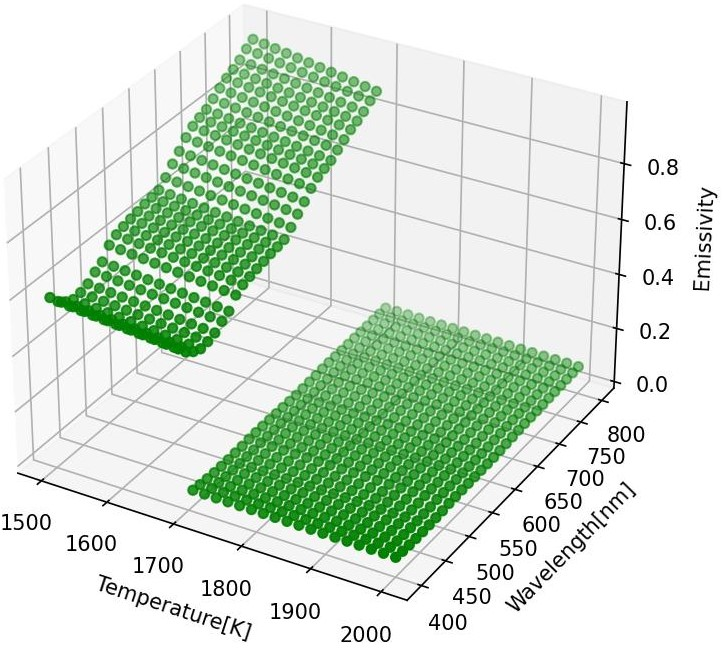
\includegraphics[width=0.6\textwidth]{figures/emissivity_model.jpg}
  \caption{Emissivity value along wavelength and temperature calculated from model 9}
  \label{fig: emissivity_model}
\end{figure}


Fig.\ref{fig: emissivity_model} shows the emissivity model based 
on model 9 in different temperature 
and wavelength. It can be found that the emissivity at a temperature 
below melting temperature ($1700K$) varies significantly with wavelength.
This is caused due to the raw emissivity data. Then, at liquid phase of 
the hypothetical material, emissivity decreases to a value lower than $0.1$.


Thus, the phase change phenomenon of hypothetical material is also characterized, 
which gives the virtual experiment platform more potential to simulate 
real experiments.


\subsection{Camera model}
After obtaining the temperature field and emissivity model of hypothetical material, 
the physical value of spectral radiation intensity should be calculated, then, 
the physical value of spectral radiation intensity is converted to 
digital value using camera model, which is the output of the complete virtual 
experiment platform. 


As mentioned in Fig.\ref{fig: received}, the camera model is based on an integration 
method, which integrate the spectral intensity received by the sensor along the 
specific range of wavelength. However, due to the varying quantum 
efficiency of each channel in sensor, it means that for a virtual camera 
with 8 channels, each pixel requires 8 independent integration operations. 
This operation requires a large computational effort. So, in order to 
accelerate the generation speed and thus reduce the time cost of virtual 
experiment platform, a parallel computing strategy is introduced.





\section{Rebuild Physical value}
\subsection{Emissivity model used for calculation}

\subsection{Curve fit algorithm}

\subsection{Parameters in calculation}
quantum efficiency, lens factor

\section{Validation}